\exercisesheader{}

% 51 - exploring_combinations_ap

\eoce{\qt{Exploring combinations\label{exploring_combinations_ap}} A coin is tossed 5 times.  How many sequences / combinations of Heads/Tails are there that have: 
\begin{parts}
\item Exactly 1 Tail?
\item Exactly 4 Tails?
\item Exactly 3 Tails?
\item At least 3 Tails?
\end{parts}
}{}

% 52 - political_affiliation_ap

\eoce{\qt{Political affiliation\label{political_affiliation_ap}}  Suppose that in a large population, 51\% identify as Democrat. A researcher takes a random sample of 3 people.
\begin{parts}
\item Use the binomial model to calculate the probability that two of them identify as Democrat.
\item Write out all possible orderings of 3 people, 2 of whom identify as Democrat. Use these scenarios to calculate the same probability from part (a) but using the Addition Rule for disjoint events. Confirm that your answers from parts (a) and (b) match.
\item If we wanted to calculate the probability that a random sample of 8 people will have 3 that identify as Democrat, briefly describe why the approach from part (b) would be more tedious than the approach from part (a).
\end{parts}
}{}

% 53 - underage_drinking_intro

\eoce{\qt{Underage drinking, Part I\label{underage_drinking_intro}}
Data collected by the Substance Abuse and Mental Health
Services Administration (SAMSHA) suggests that 69.7\% of
18-20 year olds consumed alcoholic beverages in any given
year.\footfullcite{webpage:alcohol}
\begin{parts}
\item Suppose a random sample of ten 18-20 year olds is taken. Is the use 
of the binomial distribution appropriate for calculating the probability that 
exactly six consumed alcoholic beverages? Explain.
\item Calculate the probability that exactly 6 out of 10 randomly sampled 18-
20 year olds consumed an alcoholic drink.
\item What is the probability that exactly four out of ten 18-20 year 
olds have \textit{not} consumed an alcoholic beverage?
\item What is the probability that at most 2 out of 5 randomly sampled 18-20 
year olds have consumed alcoholic beverages?
\item What is the probability that at least 1 out of 5 randomly sampled 18-20 
year olds have consumed alcoholic beverages?
\end{parts}
}{}

% 54 - chicken_pox_intro

\eoce{\qt{Chicken pox, Part I\label{chicken_pox_intro}} The National Vaccine 
Information Center estimates that 90\% of Americans have had chickenpox by 
the time they reach adulthood.  \footfullcite{webpage:chickenpox}
\begin{parts}
\item Suppose we take a random sample of 100 American adults. Is the use of 
the binomial distribution appropriate for calculating the probability that exactly 97 
out of 100 randomly sampled American adults had chickenpox during childhood? Explain.
\item Calculate the probability that exactly 97 out of 100 randomly sampled 
American adults had chickenpox during childhood.
\item What is the probability that exactly 3 out of a new sample of 100 
American adults have \textit{not} had chickenpox in their childhood?
\item What is the probability that at least 1 out of 10 randomly sampled 
American adults have had chickenpox?
\item What is the probability that at most 3 out of 10 randomly sampled 
American adults have \textit{not} had chickenpox?
\end{parts}
}{}

% 55 - dreidel

\eoce{\qt{Game of dreidel\label{dreidel}} A dreidel is a four-sided spinning top 
with the Hebrew letters \textit{nun}, \textit{gimel}, \textit{hei}, and 
\textit{shin}, one on each side. Each side is equally likely to come up in a 
single spin of the dreidel. Suppose you spin a dreidel three times. Calculate 
the probability of getting

\noindent\begin{minipage}[c]{0.45\textwidth}
\begin{parts}
\item at least one \textit{nun}? 
\item exactly 2 \textit{nun}s? 
\item exactly 1 \textit{hei}? 
\item at most 2 \textit{gimel}s? \vspace{3mm}
\end{parts}
\end{minipage}%
\begin{minipage}[c]{0.25\textwidth}
\ \vspace{2mm}

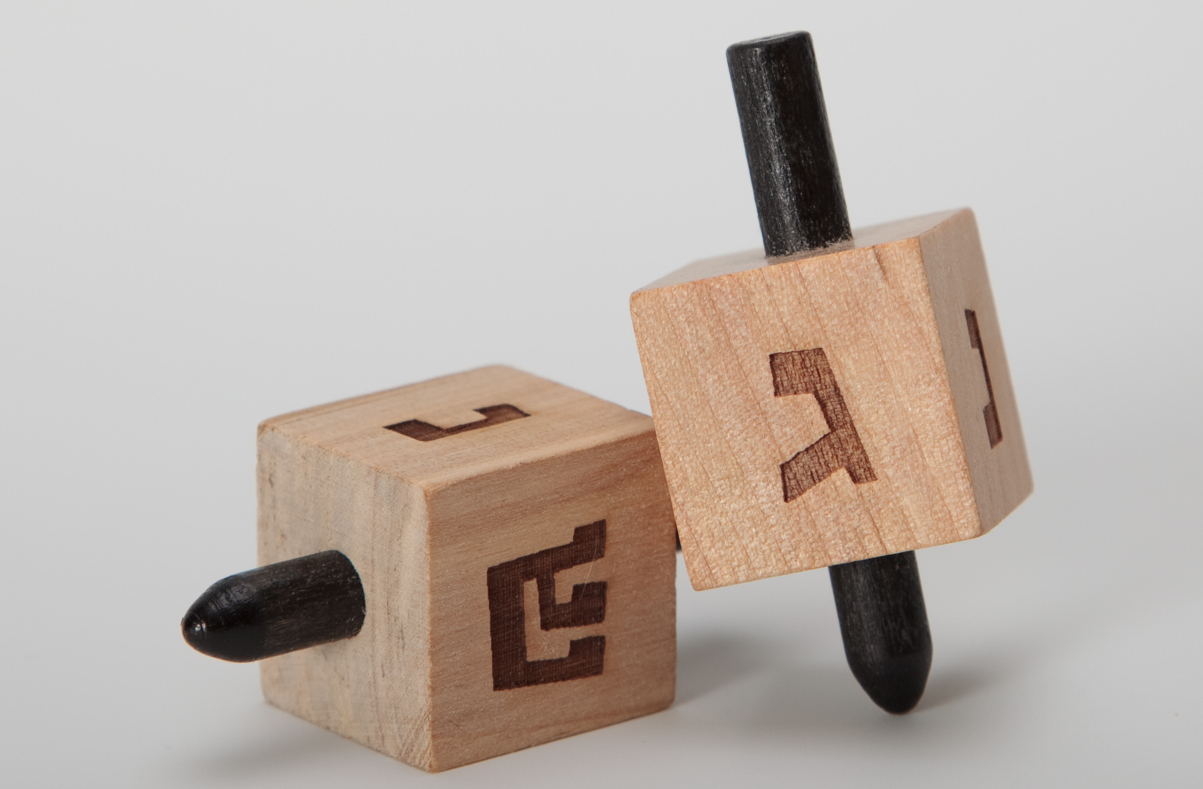
\includegraphics[width=0.95\textwidth]{ch_probability/figures/eoce/dreidel/dreidel.jpg}\vspace{2mm}
\end{minipage}%
\begin{minipage}[c]{0.28\textwidth}%
{\footnotesize Photo by Staccabees, cropped \\
  (\oiRedirect{textbook-flickr_staccabees_dreidels}{http://flic.kr/p/7gLZTf}) \\
  \oiRedirect{textbook-CC_BY_2}{CC~BY~2.0~license}} \\
\end{minipage}
}{}

% 56 - sickle_cell_anemia

\eoce{\qt{Sickle cell anemia\label{sickle_cell_anemia}} Sickle cell anemia is a 
genetic blood disorder where red blood cells lose their flexibility and 
assume an abnormal, rigid, ``sickle" shape, which results in a risk of 
various complications. If both parents are carriers of the disease, then a 
child has a 25\% chance of having the disease, 50\% chance of being a 
carrier, and 25\% chance of neither having the disease nor being a carrier. 
If two parents who are carriers of the disease have 3 children, what is the 
probability that 
\begin{parts}
\item two will have the disease?
\item none will have the disease?
\item at least one will neither have the disease nor be a carrier?
\item the first child with the disease will the be $3^{rd}$ child?
\end{parts}
}{}

% 57 - underage_drinking_normal_approx

\eoce{\qt{Underage drinking, Part II\label{underage_drinking_normal_approx}} \videosolution{underage_drinking_normal_approx}
We learned in Exercise~\ref{underage_drinking_intro}
that about 70\% of 18-20 year olds consumed alcoholic
beverages in any given year. We now consider a random 
sample of fifty 18-20 year olds.
\begin{parts}
\item How many people would you expect to have consumed alcoholic beverages? 
And with what standard deviation?
\item Would you be surprised if there were 45 or more people who have 
consumed alcoholic beverages?
\item What is the probability that 45 or more people in this sample have 
consumed alcoholic beverages? How does this probability relate to your answer 
to part (b)?
\end{parts}
}{}

% 58 - chicken_pox_normal_approx

\eoce{\qt{Chickenpox, Part II\label{chicken_pox_normal_approx}} We learned in 
Exercise~\ref{chicken_pox_intro} that about 90\% of American adults had 
chickenpox before adulthood. We now consider a random sample of 120 American 
adults.
\begin{parts}
\item How many people in this sample would you expect to have had chickenpox 
in their childhood? And with what standard deviation?
\item Would you be surprised if there were 105 people who have had chickenpox 
in their childhood?
\item What is the probability that 105 or fewer people in this sample have 
had chickenpox in their childhood? How does this probability relate to your 
answer to part (b)?
\end{parts}
}{}
